\documentclass[aspectratio=169]{beamer}
\usepackage{will_handley_beamer}
\usepackage{title_page}

% Commands
% --------
% - \arxiv{arxiv number}
% - \arxiv{<number>}            arxiv.org/abs/<number>
% - \oldarxiv{<arxiv number>}   arxiv.org/<number>
% - \doi{<doi>}                 doi.org/<doi>
% - \xkcd{<number>}             xkcd.com/<number>
% - \email{<email>}             <<email>>
% - \tthref{<website>}          <website>
% - \av[dist]{<quantity>}       <quantity>_{dist}
% - \student{<name>}{<detail>}{<photo>}

% Talk details
% ------------
\title{GPU-native nested sampling in BlackJAX}
\subtitle{Accelerating Bayesian inference to state-of-the-art levels}
\date{27$^{\text{th}}$ June 2025}

\begin{document}

\begin{frame}
    \titlepage
\end{frame}

\begin{frame}
    \frametitle{A Case Study in Astrostatistics}
    \begin{columns}
        \column{0.48\textwidth}
        \vspace{-10pt}
        \begin{block}{The Challenge: GW170817}
            \begin{itemize}
                \item \textbf{Gravitational wave detected}: Binary neutron star merger
                \item \textbf{Real-time parameter estimation}: 15+ dimensional space
                \item \textbf{Sky localization}: $\sim 30$ deg$^2$ uncertainty
                \item \textbf{EM counterpart follow-up}: Telescopes need targets within seconds to minutes
            \end{itemize}
        \end{block}
        \begin{block}{Statistical Requirements}
            \begin{itemize}
                \item \textbf{Parameter estimation}: Masses, spins, distance, sky position
                \item \textbf{Model comparison}: Signal vs noise, waveform models
            \end{itemize}
        \end{block}
        \column{0.48\textwidth}
        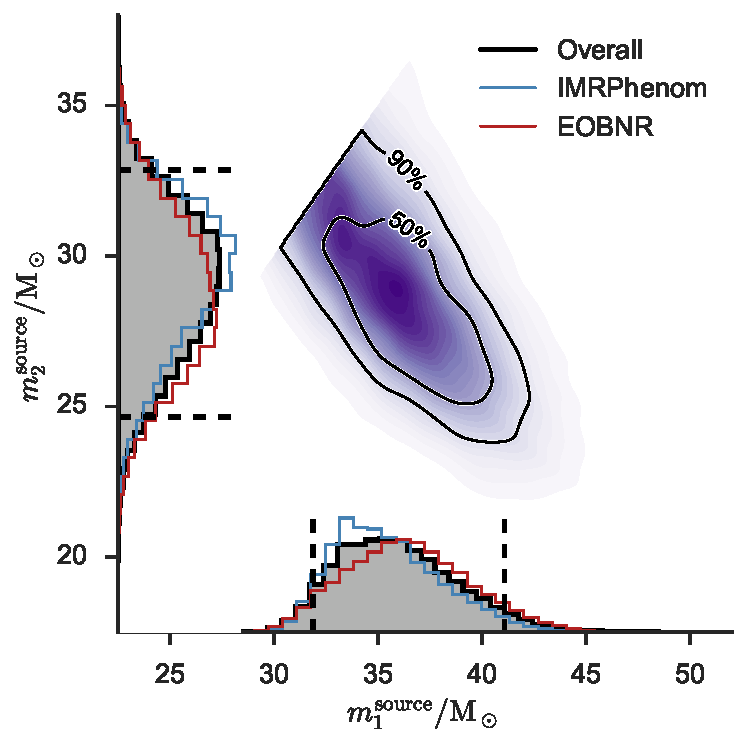
\includegraphics[height=0.49\textwidth]{figures/ligo_m1_m2}
        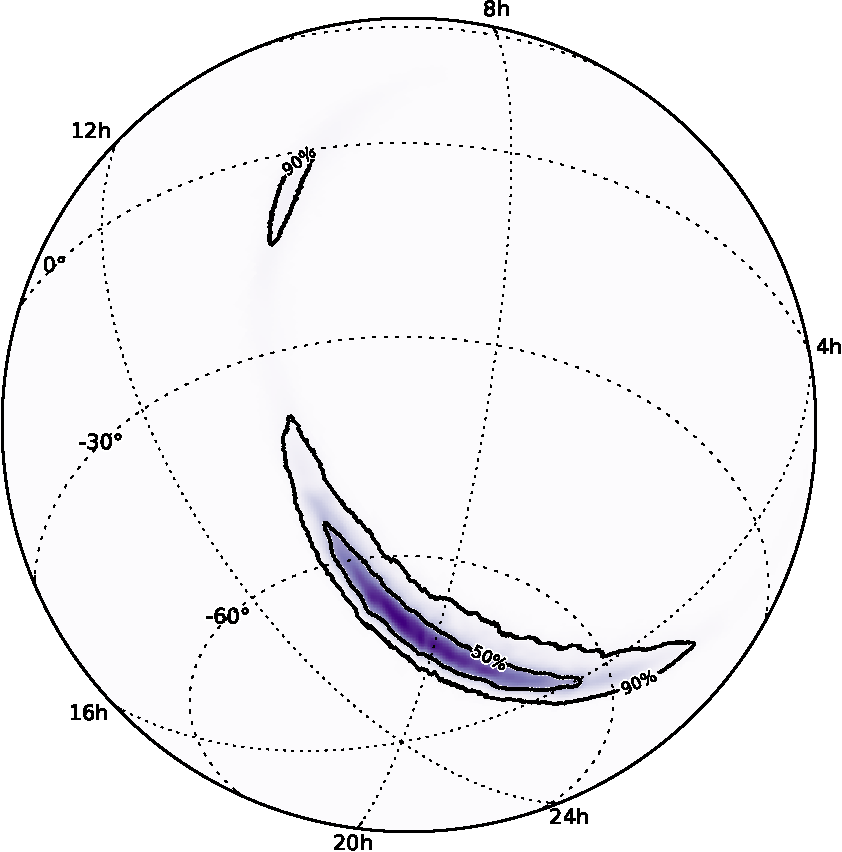
\includegraphics[height=0.49\textwidth]{figures/ligo_lambert-skymap}
        \begin{block}{The Broader Astrostatistics Context}
            \begin{itemize}
                \item \textbf{High-dimensional}: $d \sim 10^2$--$10^3$
                \item \textbf{Multimodal}: Competing physical models
                \item \textbf{Expensive likelihoods}: Complex sims
                \item \textbf{Model selection critical}: Which physics?
            \end{itemize}
        \end{block}
    \end{columns}
\end{frame}

\begin{frame}
    \frametitle{The Bayesian Inference Challenge}
    \begin{columns}
        \column{0.48\textwidth}
        \begin{block}{Parameter Estimation $P(\theta|D,M)$}
            \begin{itemize}
                \item Posterior: $\mathcal{P}(\theta|D) \propto \mathcal{L}(D|\theta) \pi(\theta)$
                \item Need samples from $\mathcal{P}(\theta|D)$
                \item Standard approach: MCMC methods
                \item Well-solved problem in many cases
            \end{itemize}
        \end{block}
        \begin{block}{Model Comparison $P(M|D)$}
            \begin{itemize}
                \item $\mathcal{Z} = \mathcal{P}(D|M) = \int \mathcal{L}(D|\theta) \pi(\theta) d\theta$
                \item Evidence/marginal likelihood/Bayes factor
                \item \textbf{Much harder to compute}
                \item MCMC doesn't estimate $\mathcal{Z}$ directly
            \end{itemize}
        \end{block}
        \column{0.48\textwidth}
        \begin{block}{Challenges for Modern Science}
            \begin{itemize}
                \item \textbf{High dimensions}: $d \sim 10^2$--$10^3$
                \item \textbf{Natural, relevant multimodality}: Multiple acceptable answers need investigation
                \item \textbf{Computational cost}: Complex forward models
                \item \textbf{Model selection}: Which physics to include?
            \end{itemize}
        \end{block}
        \begin{center}
            \textbf{Key Insight:}\\
            Need methods that compute \emph{both} \\
            posterior samples \emph{and} evidence
        \end{center}
    \end{columns}
\end{frame}

\begin{frame}
    \frametitle{Sampling Methods for Bayesian Inference}
    \begin{columns}
        \column{0.65\textwidth}
        \begin{block}{Single-Chain MCMC}
            \begin{itemize}
                \item \textbf{Metropolis-Hastings}: Simple, widely used (PyMC)
                \item \textbf{HMC/NUTS}: Gradient-based, efficient (Stan, BlackJAX)
                \item Fast for unimodal well-conditioned problems, no evidence
            \end{itemize}
        \end{block}
        \begin{block}{Ensemble Methods}
            \begin{itemize}
                \item \textbf{Affine-invariant}: emcee, zeus
                \item \textbf{Sequential Monte Carlo}: Tempering, annealing
                \item can struggle with multimodality, some estimate evidence
            \end{itemize}
        \end{block}
        \column{0.35\textwidth}
        \begin{columns}
            \column{0.5\textwidth}
        \includegraphics[width=\textwidth]{figures/emcee}
        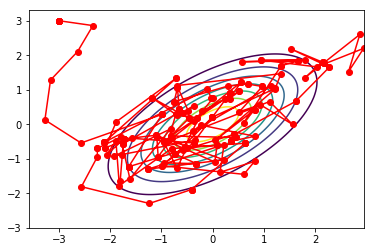
\includegraphics[width=\textwidth]{figures/metropolis-hastings}
            \column{0.5\textwidth}
        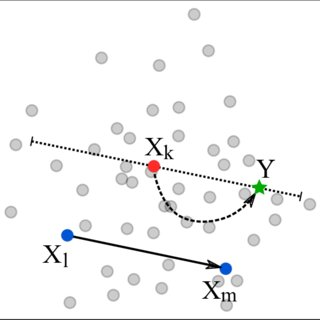
\includegraphics[width=\textwidth]{figures/zeus}
        \end{columns}
        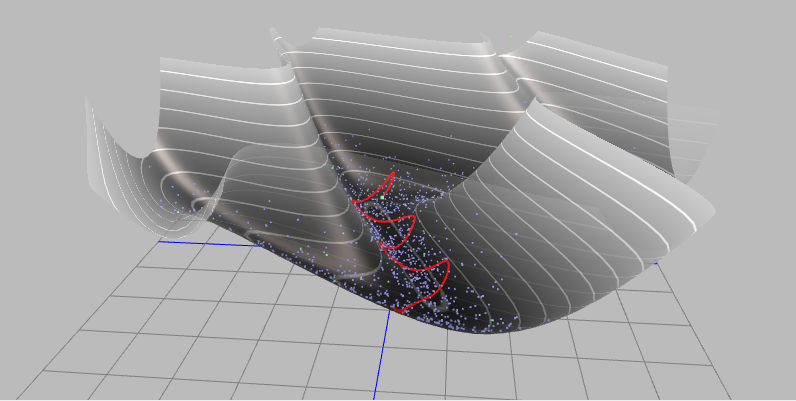
\includegraphics[width=\textwidth]{figures/hmc_explained}
        \vspace{-20pt}
        \begin{center}
            \textbf{Nested sampling}: \\
            Unique in targeting 
            evidence computation directly
        \end{center}
    \end{columns}
\end{frame}

\begin{frame}
    \begin{columns}
        \column{0.48\textwidth}
        \begin{block}{\textbf{MCMC}}
            \only<16>{
                \begin{itemize}
                    \item Single ``walker''
                    \item Explores posterior
                    \item Fast, if proposal matrix is tuned
                    \item Parameter estimation
                    \item Channel capacity optimised for generating posterior samples
                \end{itemize}
            }
        \end{block}
            \includegraphics<1>[width=\textwidth,page=1]{figures/himmelblau_mcmc}%
            \includegraphics<2>[width=\textwidth,page=2]{figures/himmelblau_mcmc}%
            \includegraphics<3>[width=\textwidth,page=3]{figures/himmelblau_mcmc}%
            \includegraphics<4>[width=\textwidth,page=4]{figures/himmelblau_mcmc}%
            \includegraphics<5>[width=\textwidth,page=5]{figures/himmelblau_mcmc}%
            \includegraphics<6-15>[width=\textwidth,page=9]{figures/himmelblau_mcmc}%
        \centerline{\includegraphics<16>[width=0.5\textwidth,page=9]{figures/himmelblau_mcmc}}%
        \column{0.48\textwidth}
        \begin{block}<7->{\textbf{Nested sampling}}
            \only<16>{
                \begin{itemize}
                    \item Ensemble of ``live points''
                    \item Scans from prior to peak of likelihood
                    \item Slower, no tuning required
                    \item Parameter estimation, model comparison
                    \item Channel capacity optimised for computing partition function
                \end{itemize}
            }
        \end{block}
            \includegraphics<7|handout:0>[width=\textwidth,page=1]{figures/himmelblau_ns}%
            \includegraphics<8|handout:0>[width=\textwidth,page=2]{figures/himmelblau_ns}%
            \includegraphics<9|handout:0>[width=\textwidth,page=3]{figures/himmelblau_ns}%
            \includegraphics<10          >[width=\textwidth,page=4]{figures/himmelblau_ns}%
            \includegraphics<11|handout:0>[width=\textwidth,page=5]{figures/himmelblau_ns}%
            \includegraphics<12|handout:0>[width=\textwidth,page=6]{figures/himmelblau_ns}%
            \includegraphics<13|handout:0>[width=\textwidth,page=7]{figures/himmelblau_ns}%
            \includegraphics<14|handout:0>[width=\textwidth,page=8]{figures/himmelblau_ns}%
            \includegraphics<15|handout:0>[width=\textwidth,page=8]{figures/himmelblau_ns}%
        \centerline{\includegraphics<16>[width=0.5\textwidth,page=4]{figures/himmelblau_ns}} %
    \end{columns}
\end{frame}

\begin{frame}
    \frametitle{The nested sampling meta-algorithm: live points}
    \begin{columns}
        \column{0.5\textwidth}
        \begin{itemize}
            \item Start with $n$ random samples over the space.
            \item Delete outermost sample, and replace with a new random one at higher integrand value.
            \item The ``live points'' steadily contract around the peak(s) of the function.
            \item We can use this evolution to estimate volume \emph{probabilistically}.
            \item At each iteration, the contours contract by $\sim\frac{1}{n}\only<5->{\pm \frac{1}{n}}$ of their volume.
            \item This is an exponential contraction, so
                \[  \int f(x) dV \approx \sum_i f(x_i) \Delta V_i, \quad V_i = V_0 e^{-\only<5->{(}i\only<5->{\pm\sqrt{i})}/n} \]
        \end{itemize}
        \column{0.5\textwidth}
        \includegraphics<1|handout:0>[width=\textwidth,page=1]{figures/himmelblau_ns}%
        \includegraphics<2|handout:0>[width=\textwidth,page=2]{figures/himmelblau_ns}%
        \includegraphics<3|handout:0>[width=\textwidth,page=3]{figures/himmelblau_ns}%
        \includegraphics<4-         >[width=\textwidth,page=4]{figures/himmelblau_ns}%
    \end{columns}
\end{frame}

\begin{frame}
    \frametitle{The nested sampling meta-algorithm: dead points}
    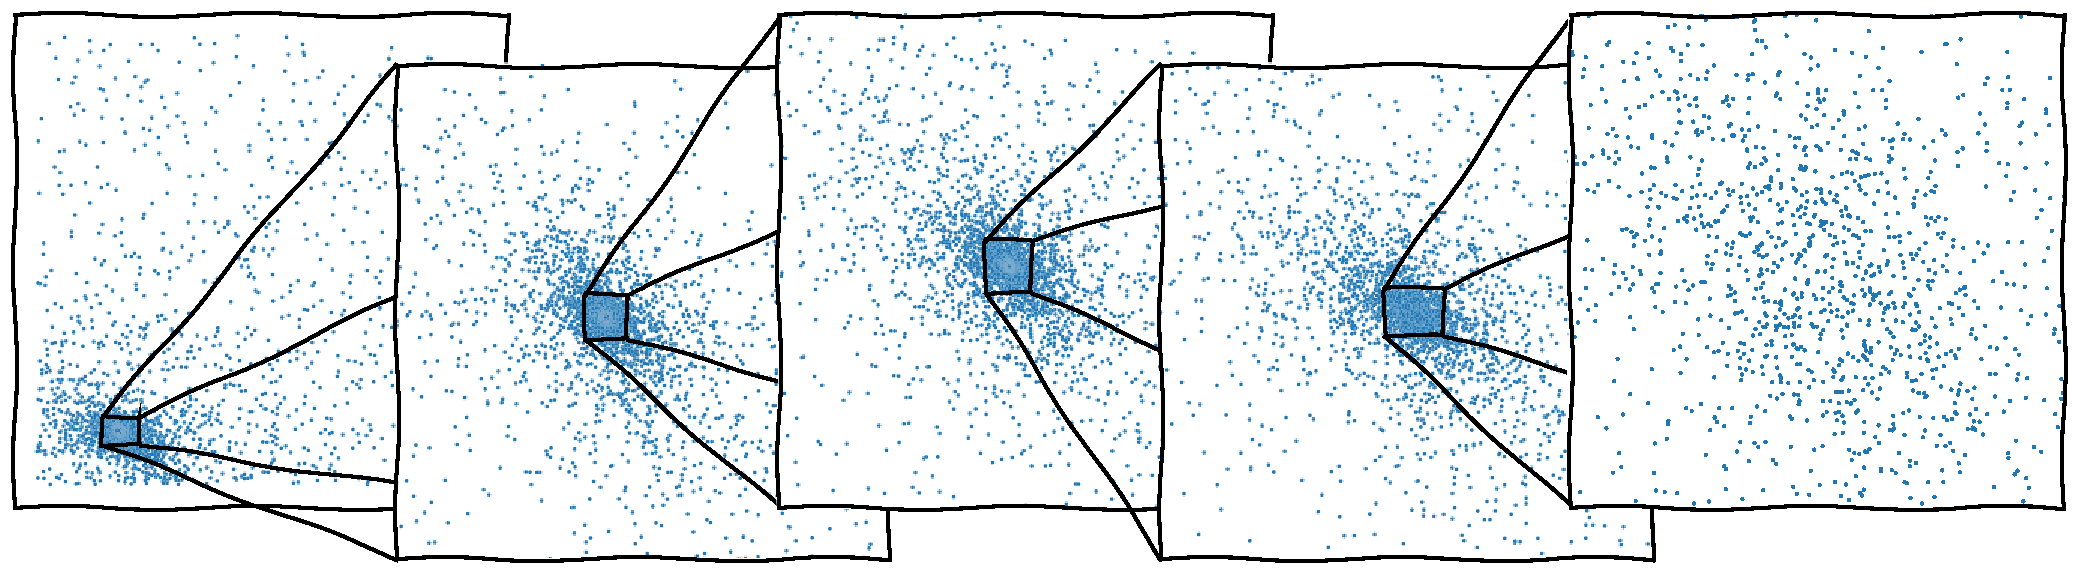
\includegraphics[width=\textwidth]{figures/dead_measure}
    \begin{columns}
        \column{0.7\textwidth}
        \begin{itemize}
            \item At the end, left with a set of discarded ``dead points''.
            \item Dead points have a unique scale-invariant distribution $\propto\: \tfrac{dV}{V}$.
            \item Each dead point gets a \textbf{posterior weight}: $w_i = \mathcal{L}_i \Delta V_i$
        \end{itemize}
        \column{0.3\textwidth}
        \begin{block}{Key Output}
        \begin{itemize}
            \item \textbf{Posterior samples} $\theta_i$ weight~$w_i=\mathcal{L}_i \Delta V_i$
            \item \textbf{Evidence} $\mathcal{Z} = \sum_i w_i$
        \end{itemize}
        \end{block}
    \end{columns}
\end{frame}

\begin{frame}
    \frametitle{Nested Sampling as Partition Function Calculator $\log \mathcal{Z}(\beta)$}
    \begin{columns}
        \column{0.48\textwidth}
        \begin{block}{The Key Insight}
            \begin{itemize}
                \item Nested sampling directly estimates the \textbf{density of states}:
                    \[ g(\mathcal{L}) = \int \delta(\mathcal{L}(\theta) - \mathcal{L}) \pi(\theta) d\theta \]
                \item This is the \textbf{partition function} at inverse temperature $\beta$:
                    \[ \mathcal{Z}(\beta) = \int g(\mathcal{L}) \mathcal{L}^{\beta} d\mathcal{L} \]
                \item Evidence is special case: $\mathcal{Z} = \mathcal{Z}(\beta=1)$
                \item \textbf{In practice}: $\mathcal{Z}(\beta) \approx \sum_i \mathcal{L}_i^\beta \Delta V_i$
            \end{itemize}
        \end{block}
        \column{0.48\textwidth}
        \begin{block}{Statistical Physics Connection}
            \begin{itemize}
                \item \textbf{Canonical ensemble}: $p(\theta|\beta) \propto \mathcal{L}(\theta)^\beta \pi(\theta)$
                \item \textbf{Free energy}: $\beta F = -\log \mathcal{Z}$
                \item \textbf{Internal energy}: $U = -\frac{\partial \log \mathcal{Z}}{\partial \beta}$
                \item \textbf{Heat capacity}: $C = \frac{\partial U}{\partial \beta}$
            \end{itemize}
        \end{block}
        \vspace{10pt}
        \begin{center}
            \textbf{Nested sampling provides the fundamental thermodynamic quantities}\\
            for any probabilistic model
        \end{center}
    \end{columns}
\end{frame}

\begin{frame}
    \frametitle{Why GPUs? The Future of High-Performance Computing}
    \begin{columns}
        \column{0.48\textwidth}
        \begin{block}{GPU Advantages (Often Confused!)}
            \begin{itemize}
                \item \textbf{Massive Parallelization}:
                    \begin{itemize}
                        \item 1000s of cores vs 10s on CPU
                        \item Perfect for ensemble algorithms
                        \item Vectorization across particles/chains
                        \item Independent likelihood evaluations
                    \end{itemize}
                \item \textbf{Automatic Differentiation}:
                    \begin{itemize}
                        \item GPU-accelerated gradients ``for free''
                        \item JAX/PyTorch ecosystem make this possible
                        \item Essential for modern optimization
                    \end{itemize}
            \end{itemize}
        \end{block}
        \column{0.48\textwidth}
        \begin{block}{The HPC Reality}
            \begin{itemize}
                \item \textbf{Future HPC is GPU dominated}:
                \item \textbf{Legacy CPU codes becoming obsolete}
            \end{itemize}
        \end{block}
        \begin{block}{Apples-to-Apples comparison}
            \begin{itemize}
                \item Quantifying GPU advantage
                    \begin{itemize}
                        \item GPUs ~40× more expensive to rent
                        \item GPUs ~100× rarer in HPC allocations
                    \end{itemize}
                \item Sometimes you don't care about walltime.
            \end{itemize}
        \end{block}
    \end{columns}
\end{frame}

\begin{frame}
    \frametitle{Why BlackJAX? Unified GPU Framework for Bayesian Inference}
    \begin{columns}
        \column{0.48\textwidth}
        \begin{block}{The Fragmentation Problem}
            \begin{itemize}
                \item \textbf{Scattered ecosystem}:
                    \texttt{MultiNest}, \texttt{PolyChord}, \texttt{dynesty}, \texttt{UltraNest}, \texttt{nautilus}, \texttt{nessai}, \ldots
            \end{itemize}
        \end{block}
        \begin{block}{BlackJAX Solution}
            \begin{itemize}
                \item \textbf{Community JAX codebase}
                \item \textbf{Fair benchmarking} with identical GPU infrastructure
                \item \textbf{Composable algorithms} with shared components
                \item \textbf{Modern ML ecosystem integration}
            \end{itemize}
        \end{block}
        \column{0.48\textwidth}
        \begin{block}{Algorithm-Hardware Matching}
            \begin{itemize}
                \item \textbf{Ensemble methods $\leftrightarrow$ GPU parallelization}:
                    \begin{itemize}
                        \item Nested sampling: 100-1000 live points
                        \item SMC: 1000s of particles
                        \item Embarrassingly parallel operations
                    \end{itemize}
                \item \textbf{Scientific problems are compute-bound}:
                    \begin{itemize}
                        \item Unlike ultra-large DL models
                        \item GPU memory rarely limiting
                        \item Perfect match for vectorization
                    \end{itemize}
            \end{itemize}
        \end{block}
    \end{columns}
\end{frame}

\begin{frame}
    \frametitle{BlackJAX Nested Slice Sampling}
    \student{david_yallup}{David Yallup}{PDRA}
    \begin{columns}
        \column{0.5\textwidth}
        \begin{block}{Core Algorithm}
            \begin{itemize}
                \item \textbf{Slice sampling} for constrained sampling
                \item Generate new live points: $\{\theta \sim \pi : \mathcal{L}(\theta) > \mathcal{L}_*\}$
                \item Vectorized operations across live points
                \item JAX transformations: \texttt{jit}, \texttt{vmap}, \texttt{grad}
            \end{itemize}
        \end{block}
        \begin{block}{GPU Advantages}
            \begin{itemize}
                \item \textbf{Parallel live points}: $n_{\text{live}} \sim 100\text{-}1000$
                \item \textbf{Vectorized slice sampling}
                \item \textbf{Batch likelihood evaluations}
                \item \textbf{Memory-efficient} on GPU
            \end{itemize}
        \end{block}
        \column{0.5\textwidth}
        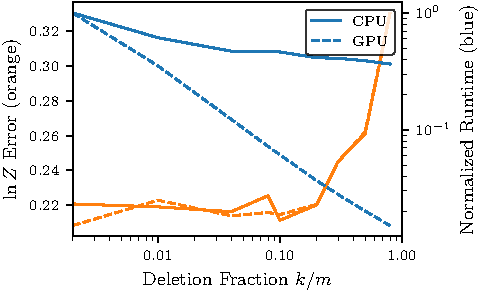
\includegraphics[width=\textwidth]{figures/scaling}
        \vspace{10pt}
        \begin{itemize}
            \item \textbf{Performance scaling}: Linear with $n_{\text{live}}$
            \item \textbf{GPU speedup}: $10\times$-$100\times$ vs CPU
            \item \textbf{Memory usage}: Constant per live point
        \end{itemize}
    \end{columns}
\end{frame}

\begin{frame}
    \frametitle{GW150914 Binary Black Hole Merger}
    \student{metha_prathaban}{Metha Prathaban}{PhD}
    \begin{columns}
        \column{0.5\textwidth}
        \begin{block}{Performance on Real Data}
            \begin{itemize}
                \item \textbf{BlackJAX GPU-NS}: 207 seconds (1 GPU)
                \item \textbf{FlowMC (GPU MCMC)}: 742 seconds (1 GPU)
                \item \textbf{Bilby/Dynesty}: ~2 hours (400 CPUs)
            \end{itemize}
            \begin{center}
                \textbf{Orders of magnitude speedup over CPU}\\
                \textbf{Comparable to other GPU-native methods}
            \end{center}
            \vspace{5pt}
        \end{block}
        \begin{block}{Key Achievement}
            \begin{itemize}
                \item Nested sampling now competitive on GPUs
                \item Direct evidence computation included
            \end{itemize}
        \end{block}
        \column{0.5\textwidth}
        \includegraphics[width=\textwidth]{materials/gw/data/GW150914_corner.pdf}
        \vspace{5pt}
        \begin{center}
            \small{Good agreement between BlackJAX\\and FlowMC posteriors}
        \end{center}
    \end{columns}
\end{frame}

\begin{frame}
    \frametitle{CMB \& Cosmic Shear Analysis}
    \student{toby_lovick}{Toby Lovick}{PhD}
    \begin{columns}
        \column{0.55\textwidth}
        \begin{block}{CMB Power Spectrum (6 params)}
            \begin{itemize}
                \item \textbf{PolyChord (CPU)}: ~1 hour
                \item \textbf{BlackJAX (GPU)}: 12 seconds
            \end{itemize}
            \begin{center}
                \textbf{300× speedup}
            \end{center}
        \end{block}
        \begin{block}{Cosmic Shear (37 params)}
            \begin{itemize}
                \item \textbf{PolyChord (48 CPUs)}: ~8 months
                \item \textbf{NUTS (12 A100 GPUs)}: 2 days
                \item \textbf{BlackJAX (1 A100 GPU)}: 4.5 hours
            \end{itemize}
            \begin{center}
                \textbf{$>$1000× speedup vs CPU}\\
                \textbf{10× speedup vs existing GPU approach}\arxiv{2405.12965}
            \end{center}
        \end{block}
        \column{0.45\textwidth}
        \includegraphics<1>[width=\textwidth]{materials/cmb_wl/CMB.pdf}%
        \includegraphics<2>[width=\textwidth]{materials/cmb_wl/jaxLCDM.pdf}
    \end{columns}
\end{frame}

\begin{frame}
    \frametitle{The Real AI Revolution: LLMs as the Missing Piece}
    \begin{columns}
        \column{0.48\textwidth}
        \begin{block}{LLMs: The GPU Code Translator}
            \begin{itemize}
                \item Automated translation: Fortran/C++ $\rightarrow$ JAX/PyTorch
                \item Bridges the gap between legacy science and modern hardware
            \end{itemize}
        \end{block}
        \begin{block}{The 80/20 Rule of Scientific Work}
            \begin{itemize}
                \item \textbf{80\% ``boring'' tasks}: forms, papers, grants, reviews, grading, code writing\ldots
                \item \textbf{20\% hard thinking}: Novel insights, experimental design, theory
                \item \textbf{AI's biggest impact}: Automating the 80\%, not the 20\%
            \end{itemize}
        \end{block}
        \column{0.48\textwidth}
        \begin{block}{Beyond Scientific Analysis}
            \begin{itemize}
                \item \textbf{Common focus}: Using LLMs for analysis
                \item \textbf{Real transformation}: Automating workflow
                \item \textbf{Already happening}:
                    \begin{itemize}
                        \item Grant writing assistance
                        \item Paper drafting and review
                        \item Code generation and debugging
                        \item Literature review automation
                    \end{itemize}
            \end{itemize}
        \end{block}
        \begin{block}{The Productivity Explosion}
            \begin{itemize}
                \item \textbf{Quality control}: Becomes the limiting factor
                \item \textbf{Focus shift}: writing $\rightarrow$ critical thinking
            \end{itemize}
        \end{block}
    \end{columns}
\end{frame}

\begin{frame}
    \frametitle{Resources}
    \begin{itemize}
        \item \textbf{Installation}: \texttt{pip install git+https://github.com/handley-lab/blackjax}
        \item \textbf{Documentation}: \tthref{handley-lab.co.uk/nested-sampling-book}
    \end{itemize}
    \begin{columns}
        \column{0.48\textwidth}
        \begin{block}{BlackJAX Implementation}
            \begin{itemize}
                \item \textbf{BlackJAX}: \github{handley-lab/blackjax}
                \item \textbf{Nested sampling}: In PR to \github{blackjax-devs/blackjax} \#755
            \end{itemize}
        \end{block}
        \begin{block}{Theory \& Background}
            \begin{itemize}
                \item \textbf{Review papers}: \arxiv{2205.15570}, \arxiv{2101.09675}
                \item \textbf{Original paper}: \citehref{https://projecteuclid.org/journals/bayesian-analysis/volume-1/issue-4/Nested-sampling-for-general-Bayesian-computation/10.1214/06-BA127.full}{}{Skilling (2006)}
            \end{itemize}
        \end{block}
        \column{0.48\textwidth}
        \begin{block}{Workshop \& Learning}
            \begin{itemize}
                \item \textbf{GPU Nested Sampling Workshop}: \tthref{github.com/handley-lab/workshop}
                \item \textbf{Interactive tutorials}: JAX, BlackJAX, GPU acceleration
            \end{itemize}
        \end{block}
    \end{columns}
\end{frame}

\begin{frame}
    \frametitle{Conclusions}
    \framesubtitle{\tthref{github.com/handley-lab/group}}
    \tikz[overlay,remember picture]
        \node[anchor=north east] (A) at ($(current page.north east)+(0,0)$) {
        
\includegraphics[width=0.09\textheight]{people/adam_ormondroyd.jpg}%
        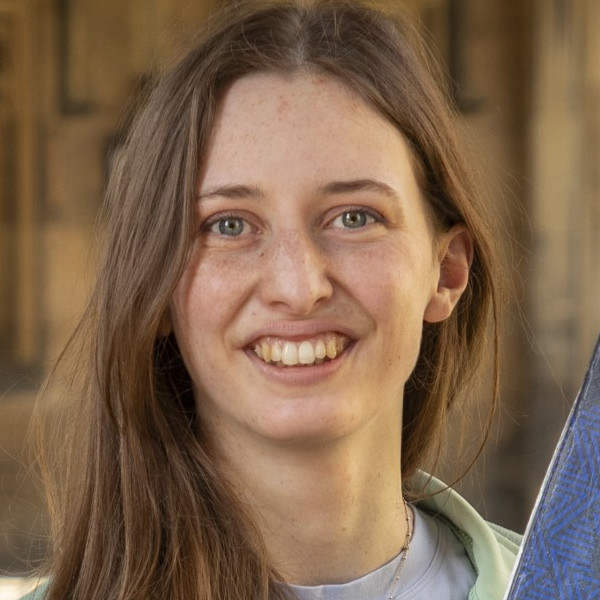
\includegraphics[width=0.09\textheight]{people/charlotte_priestley.jpg}%
        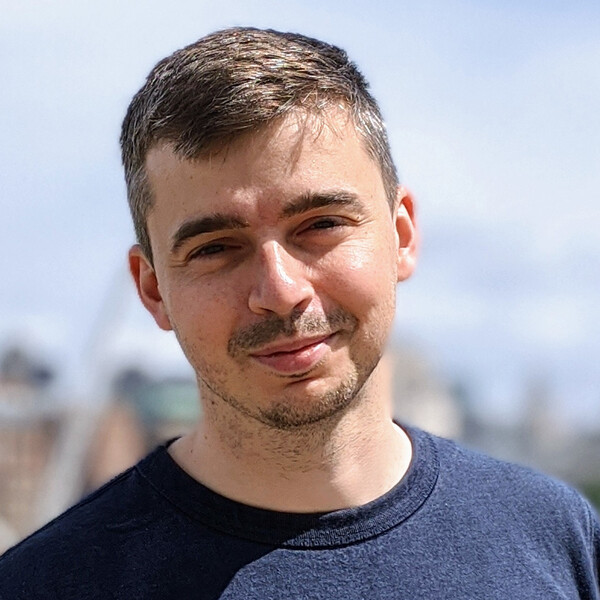
\includegraphics[width=0.09\textheight]{people/david_yallup.jpg}%
        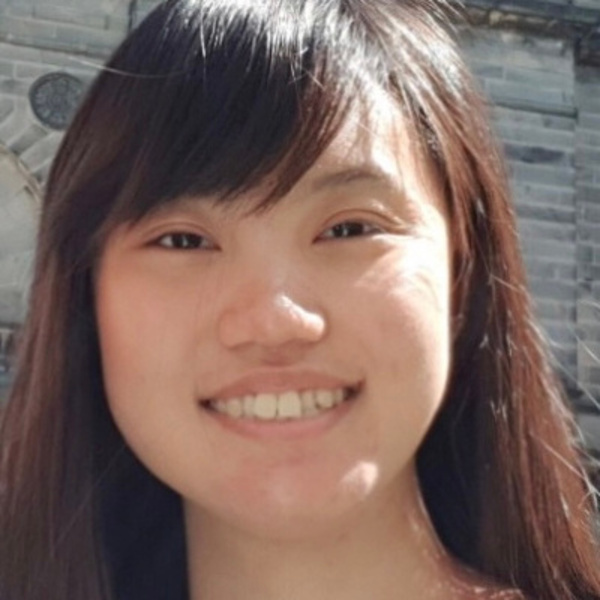
\includegraphics[width=0.09\textheight]{people/dily_ong.jpg}%
        
\includegraphics[width=0.09\textheight]{people/harry_bevins.jpg}%
        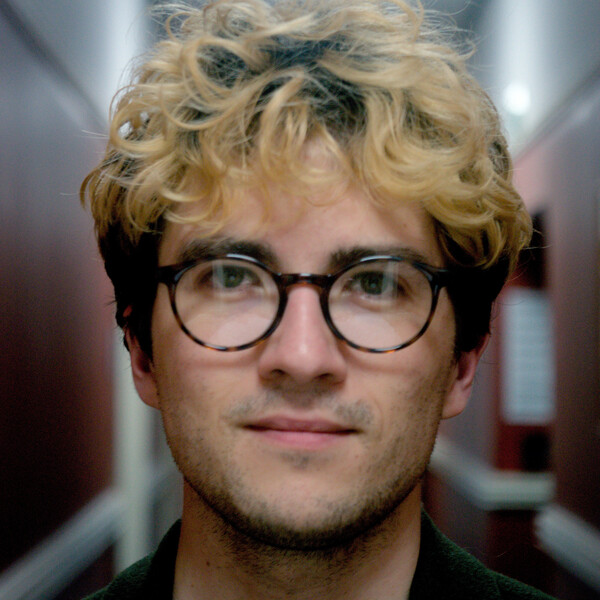
\includegraphics[width=0.09\textheight]{people/harvey_williams.jpg}%
        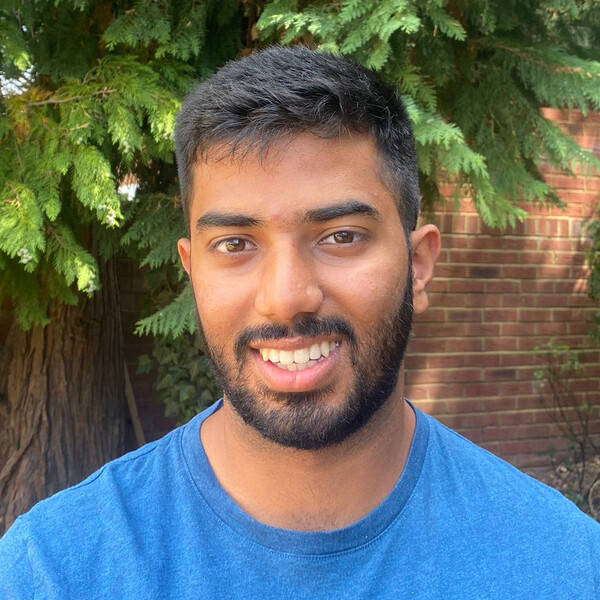
\includegraphics[width=0.09\textheight]{people/krish_nanavati.jpg}%
        
\includegraphics[width=0.09\textheight]{people/metha_prathaban.jpg}%
        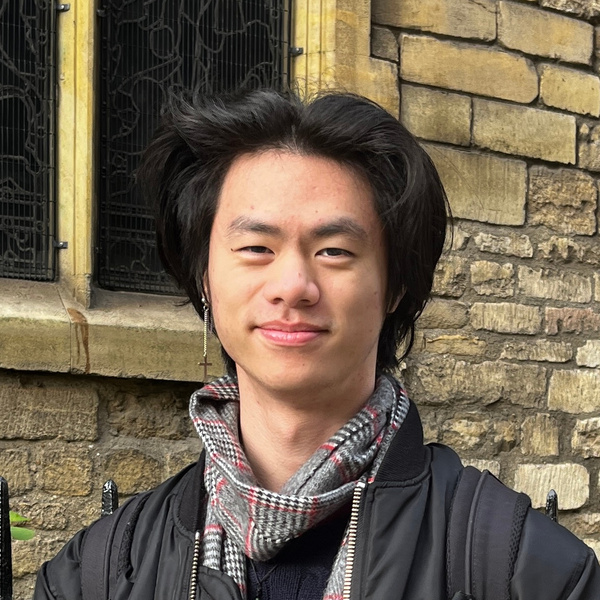
\includegraphics[width=0.09\textheight]{people/ming_yang.jpg}%
        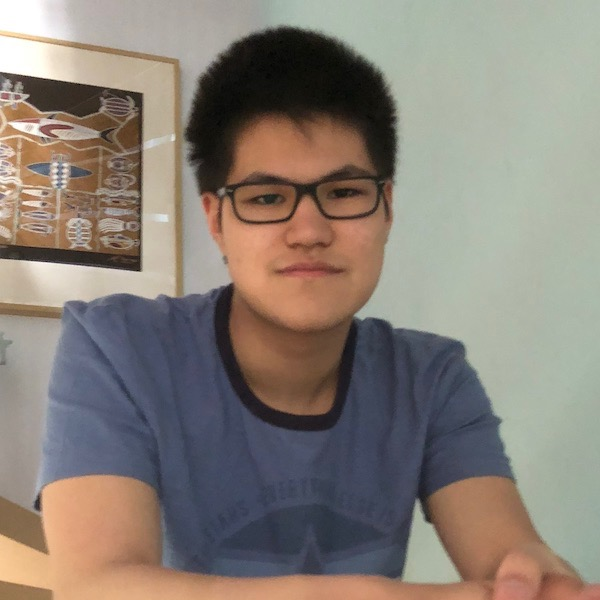
\includegraphics[width=0.09\textheight]{people/namu_kroupa.jpg}%
        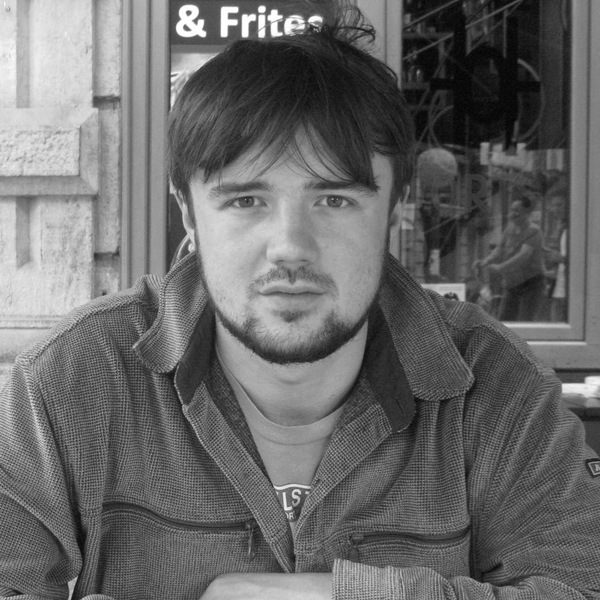
\includegraphics[width=0.09\textheight]{people/sam_leeney.jpg}%
        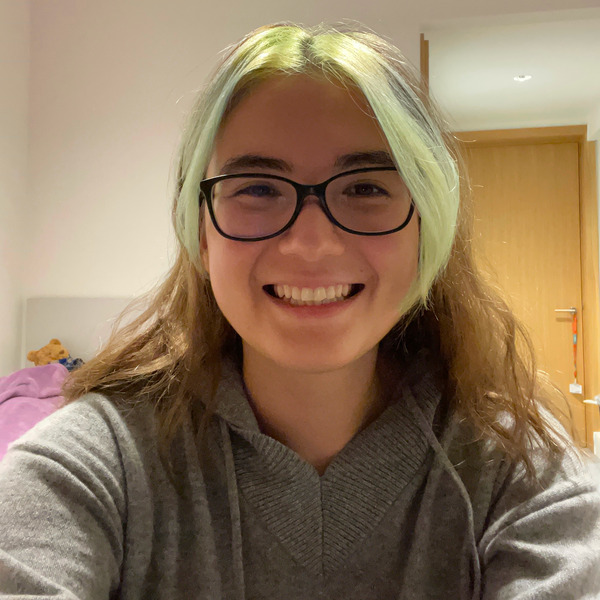
\includegraphics[width=0.09\textheight]{people/sinah_legner.jpg}%
        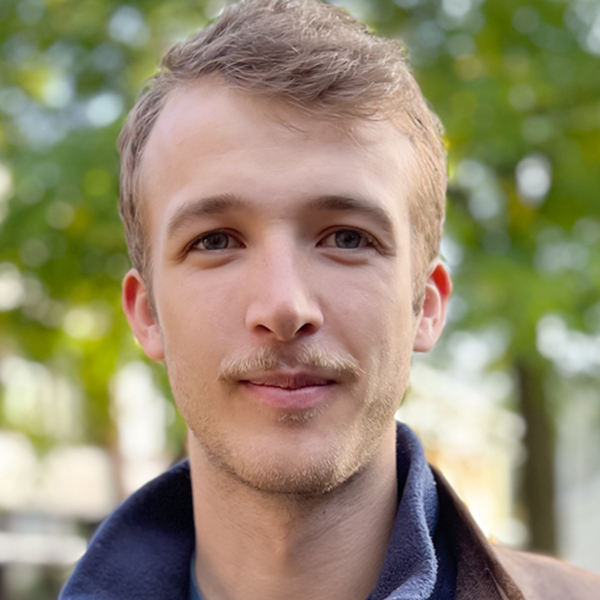
\includegraphics[width=0.09\textheight]{people/toby_lovick.jpg}%
        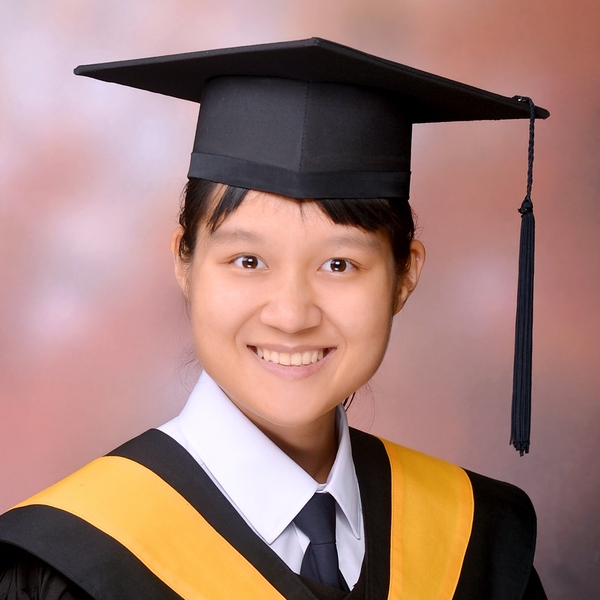
\includegraphics[width=0.09\textheight]{people/wei-ning_deng.jpg}%
        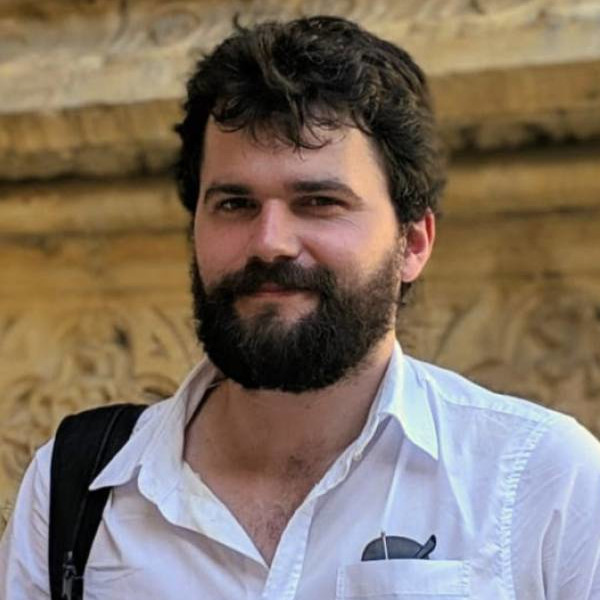
\includegraphics[width=0.09\textheight]{people/will_handley.jpg}%
        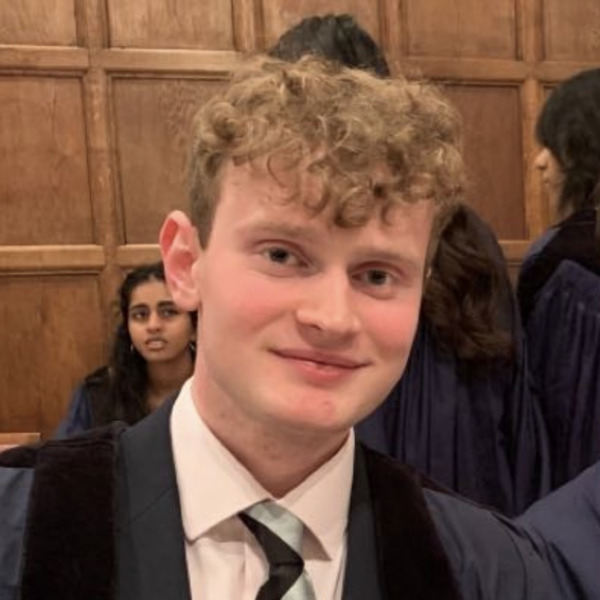
\includegraphics[width=0.09\textheight]{people/will_templeton.jpg}%
    };
    \vspace{-0.1\textheight}
    \begin{itemize}
        \item \textbf{Nested sampling is widely used} across physical sciences for parameter estimation and model comparison
        \item \textbf{BlackJAX provides GPU-native implementation} with $10\times$-$100\times$ speedups
        \item \textbf{JAX ecosystem integration} enables modern scientific workflows
        \item \textbf{Real applications} from gravitational waves to cosmology benefit immediately
        \item \textbf{The future is GPU-accelerated} scientific computing with AI integration
    \end{itemize}
\end{frame}

% Appendix
\appendix

\begin{frame}
    \frametitle{Appendix: Sequential Monte Carlo Connection}
    \begin{columns}
        \column{0.48\textwidth}
        \begin{block}{SMC Framework}
            \begin{itemize}
                \item Rigorous statistical foundation
                \item Tempered distributions: $p_t(\theta) \propto \mathcal{L}(\theta)^{\beta_t} \pi(\theta)$
                \item Nested sampling as special case of SMC
                \item Adaptive temperature schedules
            \end{itemize}
        \end{block}
        \begin{block}{Key Differences}
            \begin{itemize}
                \item \textbf{SMC}: Annealing in temperature $\beta_t$
                \item \textbf{NS}: Annealing in likelihood threshold $\mathcal{L}_*$
                \item \textbf{SMC}: Flexible inner kernels
                \item \textbf{NS}: Specialized for constrained sampling
            \end{itemize}
        \end{block}
        \column{0.48\textwidth}
        \begin{block}{BlackJAX Implementation}
            \begin{itemize}
                \item Direct comparison possible:
                    \begin{itemize}
                        \item Same GPU codebase
                        \item Identical likelihood evaluations
                        \item Fair benchmarking
                    \end{itemize}
                \item SMC with adaptive tempering
                \item Nested sampling with slice sampling
                \item Both estimate evidence $\mathcal{Z}$
            \end{itemize}
        \end{block}
        \vspace{10pt}
        \begin{center}
            \textbf{Perspective:}\\
            Statistics community: NS $\subset$ SMC\\
            Physics community: SMC $\approx$ NS variant
        \end{center}
    \end{columns}
\end{frame}

\end{document}
